\documentclass[aspectratio=169,11pt]{beamer}

% --- Packages ----------------------------------------------------------------
\usepackage[T1]{fontenc}
\usepackage[utf8]{inputenc}
\usepackage{lmodern}
\usepackage{microtype}
\usepackage{graphicx}
\usepackage{xcolor}
\usepackage{booktabs}
\usepackage{tabularx}
\usepackage{tikz}
\usepackage{listings}

\usetikzlibrary{positioning,shapes.geometric,arrows.meta,calc,fit,backgrounds}

% --- Theme: clean, paper-like (matches the article) -------------------------
\usetheme{default}
\usecolortheme{default}
\beamertemplatenavigationsymbolsempty
\setbeamertemplate{footline}{%
  \hfill{\scriptsize\color{black!50}\insertframenumber\,/\,\inserttotalframenumber}\hspace*{4mm}\vspace*{2mm}%
}
\setbeamercolor{structure}{fg=blue!50!black}
\setbeamercolor{frametitle}{fg=blue!50!black,bg=white}
\setbeamercolor{title}{fg=blue!50!black}
\setbeamercolor{subtitle}{fg=black!75}
\setbeamercolor{author}{fg=black!75}
\setbeamercolor{date}{fg=black!75}
\setbeamerfont{frametitle}{series=\bfseries}
\setbeamerfont{title}{series=\bfseries,size=\Large}
\setbeamercolor{itemize item}{fg=blue!50!black}
\setbeamercolor{itemize subitem}{fg=blue!50!black}
\setbeamercolor{enumerate item}{fg=blue!50!black}
\setbeamercolor{block title}{fg=white,bg=blue!50!black}
\setbeamercolor{block body}{bg=blue!4}
\setbeamertemplate{itemize item}{\textbullet}
\setbeamertemplate{itemize subitem}{\textendash}

% --- Listings (matches report) ----------------------------------------------
\definecolor{codebg}{RGB}{246,248,250}
\definecolor{codecmt}{RGB}{106,115,125}
\definecolor{codekw}{RGB}{215,58,73}
\definecolor{codestr}{RGB}{32,113,69}

\lstdefinestyle{py}{
  backgroundcolor=\color{codebg},
  basicstyle=\ttfamily\scriptsize,
  commentstyle=\color{codecmt}\itshape,
  keywordstyle=\color{codekw}\bfseries,
  stringstyle=\color{codestr},
  language=Python,
  numbers=none,
  breaklines=true,
  frame=single,
  framesep=4pt,
  rulecolor=\color{black!18},
  showstringspaces=false,
  tabsize=2,
}

\graphicspath{{../report/figures/}}

% --- Title -------------------------------------------------------------------
\title[Enterprise Doc AI]{\textbf{Enterprise Doc AI}}
\subtitle{A Local-First Retrieval-Augmented Generation System\\for Private Document Question Answering}
\author{Shahab Azmi}
\date{May 2026}

\begin{document}

% =============================================================================
\begin{frame}[plain]
  \titlepage
\end{frame}

% --- Slide 2: Motivation -----------------------------------------------------
\begin{frame}{Motivation}
\begin{itemize}\setlength{\itemsep}{4pt}
  \item Hosted LLMs cannot be trusted with confidential material -- contracts,
        exam papers, internal HR documents.
  \item Generic LLMs hallucinate; hosted RAG services are opaque about
        \emph{which passages} grounded an answer.
  \item Paid APIs are metered: every page indexed and every query has a unit cost.
\end{itemize}
\medskip
\begin{block}{Thesis}
\textit{Push RAG to its local-first limit.} Parser, embedder, BM25 index, vector
store, generator and conversation memory all run on a single Apple\,M2
(8\,GB RAM, no GPU, no internet at query time).
\end{block}
\end{frame}

% --- Slide 3: Contributions --------------------------------------------------
\begin{frame}{Contributions}
\begin{enumerate}\setlength{\itemsep}{3pt}
  \item A complete, runnable \textbf{local-first RAG pipeline} -- BGE bi-encoder,
        Okapi BM25, and a 3\,B Q4-quantised generator served by Ollama.
  \item A \textbf{seven-class query classifier} that routes each query to a
        different prompt template, retrieval depth, and token budget.
        \emph{Two of seven classes bypass the LLM entirely.}
  \item A \textbf{hybrid reranker} fusing normalised BM25 and dense ranks, plus
        small domain-aware bonuses tuned for personal-document corpora.
  \item A \textbf{table-aware chunker} that detects high-density numeric line
        patterns and preserves their structure for retrieval over financial PDFs.
  \item A \textbf{persistence design} where SQLite is the single source of truth
        and the embedded vector store is rebuilt from it on startup.
\end{enumerate}
\end{frame}

% --- Slide 4: Architecture ---------------------------------------------------
\begin{frame}{System Architecture}
\centering
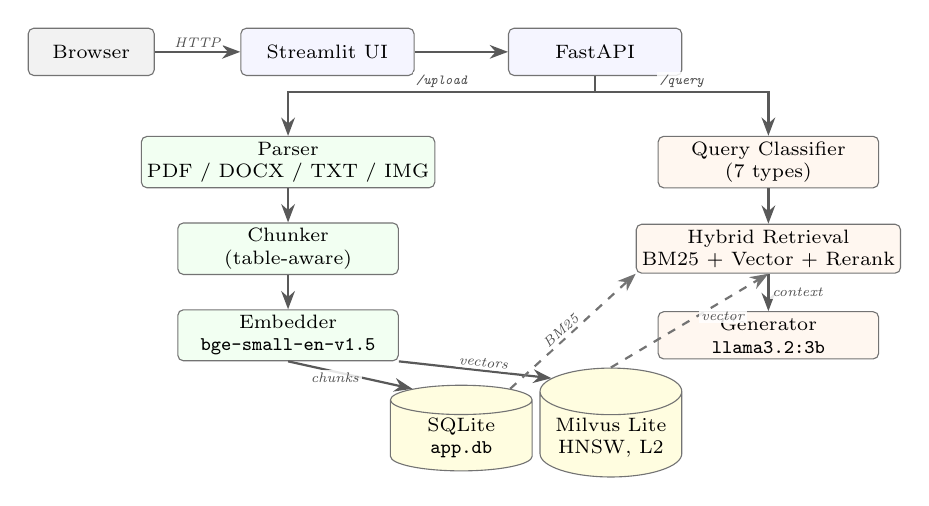
\begin{tikzpicture}[
  every node/.style={font=\scriptsize,align=center},
  block/.style={rectangle,draw=black!55,rounded corners=2pt,minimum width=22mm,
                minimum height=6mm,inner sep=2pt,fill=blue!4},
  ingblk/.style={rectangle,draw=black!55,rounded corners=2pt,minimum width=28mm,
                 minimum height=6mm,inner sep=2pt,fill=green!5},
  qryblk/.style={rectangle,draw=black!55,rounded corners=2pt,minimum width=28mm,
                 minimum height=6mm,inner sep=2pt,fill=orange!6},
  store/.style={cylinder,shape border rotate=90,draw=black!55,minimum width=18mm,
                minimum height=8mm,inner sep=1pt,aspect=0.4,fill=yellow!12},
  user/.style ={rectangle,rounded corners=2pt,draw=black!55,minimum width=16mm,
                minimum height=6mm,fill=gray!10},
  arr/.style  ={-Stealth,thick,black!65},
  rdarr/.style={-Stealth,thick,black!55,dashed},
  lab/.style  ={font=\tiny\itshape,black!70,inner sep=1pt,fill=white,
                fill opacity=0.85,text opacity=1},
]
\node[user]   at (0,    0)    (browser)   {Browser};
\node[block]  at (3.0,  0)    (st)        {Streamlit UI};
\node[block]  at (6.4,  0)    (api)       {FastAPI};

\node[ingblk] at (2.5, -1.4)  (parse)     {Parser\\PDF / DOCX / TXT / IMG};
\node[ingblk] at (2.5, -2.5)  (chunk)     {Chunker\\(table-aware)};
\node[ingblk] at (2.5, -3.6)  (embed)     {Embedder\\\texttt{bge-small-en-v1.5}};

\node[qryblk] at (8.6, -1.4)  (classify)  {Query Classifier\\(7 types)};
\node[qryblk] at (8.6, -2.5)  (retrieve)  {Hybrid Retrieval\\BM25 + Vector + Rerank};
\node[qryblk] at (8.6, -3.6)  (gen)       {Generator\\\texttt{llama3.2:3b}};

\node[store]  at (4.7, -4.9)  (sqlite)    {SQLite\\\texttt{app.db}};
\node[store]  at (6.6, -4.9)  (milvus)    {Milvus Lite\\HNSW, L2};

\draw[arr] (browser.east) -- node[lab,above]{HTTP} (st.west);
\draw[arr] (st.east)      -- (api.west);
\draw[arr] (api.south) -- ++(0,-2mm) -|
  node[lab,pos=0.25,above]{\texttt{/upload}} (parse.north);
\draw[arr] (api.south) -- ++(0,-2mm) -|
  node[lab,pos=0.25,above]{\texttt{/query}}  (classify.north);
\draw[arr] (parse)    -- (chunk);
\draw[arr] (chunk)    -- (embed);
\draw[arr] (classify) -- (retrieve);
\draw[arr] (retrieve) -- node[lab,right]{context} (gen);
\draw[arr] (embed.south)
  -- node[lab,left,pos=0.6]{chunks} (sqlite.north west);
\draw[arr] (embed.south east)
  -- node[lab,above,sloped,pos=0.55]{vectors} (milvus.north west);
\draw[rdarr] (sqlite.north east)
  -- node[lab,above,sloped,pos=0.45]{BM25} (retrieve.south west);
\draw[rdarr] (milvus.north)
  -- node[lab,right,pos=0.55]{vector} (retrieve.south);
\end{tikzpicture}

\smallskip
{\scriptsize Solid arrows = write; dashed = read.\quad
\textcolor{green!40!black}{Green}: ingest pipeline.\quad
\textcolor{orange!70!black}{Orange}: query pipeline.\quad
SQLite is the single source of truth.}
\end{frame}

% --- Slide 5: Table-aware Chunking ------------------------------------------
\begin{frame}[fragile]{Implementation: Table-aware Chunking}
\textbf{Problem.} Naive whitespace collapsing destroys tables -- rows and columns merge
into a single line, hurting both BM25 and vector retrieval scores.
\smallskip

\textbf{Heuristic.} If $\geq 3$ lines exist and $> 40\,\%$ are short ($<\!80$ chars)
\emph{and} contain a digit, treat the chunk as tabular: keep line breaks, collapse only
intra-line whitespace.
\smallskip

\begin{lstlisting}[style=py]
def _normalize_chunk_text(text):
    lines = [l for l in text.split("\n") if l.strip()]
    numeric_short = sum(1 for l in lines
                        if len(l.strip()) < 80 and any(c.isdigit() for c in l))
    if len(lines) >= 3 and numeric_short / len(lines) > 0.4:
        return "\n".join(" ".join(l.split()) for l in lines)   # table mode
    return " ".join(text.split())                              # prose mode
\end{lstlisting}
\smallskip

{\small Added after observing that \textit{Tesla, Inc.\ Form 10-K} pages produced
unreadable single-line chunks before normalisation -- which severely hurt retrieval over
the 633-chunk financial PDF.}
\end{frame}

% --- Slide 6: Hybrid Retrieval -----------------------------------------------
\begin{frame}{Hybrid Retrieval}
Four-stage pipeline (\texttt{backend/services/retrieval.py}):
\begin{enumerate}\setlength{\itemsep}{2pt}
  \item Stop-word removal $+$ alias expansion
        (\texttt{professor} $\to$ \{\texttt{prof, instructor, lecturer, teacher}\}).
  \item \textbf{Lexical}: BM25\,Okapi over chunk tokens -- top $\max(3k,12)$ candidates.
  \item \textbf{Dense}: Milvus Lite (HNSW, L2), top $\max(4k,16)$ candidates;
        L2 distance $> 1.2$ discarded as too weak.
  \item \textbf{Rerank}:
        \[
          \mathrm{score}(d) \;=\; w_b \cdot \widehat{b}(d) \;+\; (1-w_b) \cdot \widehat{r}(d) \;+\; \beta(q,d)
        \]
\end{enumerate}
\smallskip
\begin{block}{Domain bonuses ($\beta$, $+0.10$\,--\,$+0.18$)}
Page-1 boost for instructor queries; \texttt{@}-token bonus for contact queries;
parenthetical-acronym bonus (``NLP'' matches ``Natural Language Processing (NLP)'');
$w_b{=}0.7$ for \textsc{numerical} queries (exact terms outweigh semantics).
\end{block}
\end{frame}

% --- Slide 6: Query Classification ------------------------------------------
\begin{frame}{Query Classification: 7 Types}
\centering\small
\begin{tabularx}{\linewidth}{@{}lccccX@{}}
\toprule
Type & $k$ & $w_b$ & $n_{\text{predict}}$ & LLM? & Triggers \\
\midrule
\textsc{extractive} & 7 & 0.5 & 250 & \textbf{no}  & ``exact paragraph'', ``verbatim'' \\
\textsc{provenance} & 3 & 0.5 & 60  & \textbf{no}  & ``which page'', ``where in'' \\
\textsc{numerical}  & 5 & 0.7 & 60  & yes & ``how many'', ``percentage'' \\
\textsc{list}       & 5 & 0.6 & 150 & yes & ``list all'', ``enumerate'' \\
\textsc{reasoning}  & 5 & 0.4 & 120 & yes & ``why does'', ``analyse'' \\
\textsc{summary}    & 6 & 0.5 & 300 & yes & ``summarise'', ``key points'' \\
\textsc{factual}    & 3 & 0.5 & 120 & yes & default \\
\bottomrule
\end{tabularx}
\medskip
\begin{block}{LLM-bypass}
\textsc{Extractive} returns the top chunk verbatim; \textsc{provenance} returns only
metadata (file / page / section). Skipping the generator removes 5\,--\,10\,s of latency
and eliminates the risk of a 3\,B model paraphrasing a quote.
\end{block}
\end{frame}

% --- Slide 7: Generation -----------------------------------------------------
\begin{frame}{Generation \& Prompt Engineering}
Single Ollama call per query, \texttt{temperature}~$=0$. Prompt $=$ five-rule core
$+$ type-specific addendum.
\medskip

\textbf{Five-rule core}
\begin{itemize}\setlength{\itemsep}{1pt}
  \item Use only the retrieved context; reply ``Not found in document.'' when context is silent.
  \item Stop after one answer; prefer exact wording; cap at 3\,--\,4 sentences unless asked otherwise.
\end{itemize}

\textbf{Type addenda} block specific failure modes -- e.g.\ \textsc{reasoning} forbids
hedge phrases (``could lead to'', ``analysts believe'') the model would otherwise invent.
\medskip
\begin{block}{Empirical finding}
The retrieved context is concatenated with a \textbf{3000-character cap}.
Filling the model's full $\sim$4\,k context window with chunks \emph{degraded} answer quality
on the 3\,B model -- a longer context was a worse context, not a better one.
\end{block}
\end{frame}

% --- Slide 8: Evaluation -----------------------------------------------------
\begin{frame}{Evaluation}
\begin{columns}[T,onlytextwidth]
\begin{column}{0.46\textwidth}
\textbf{Corpus} (660 chunks total)
\smallskip

{\small
\begin{tabularx}{\linewidth}{@{}Xr@{}}
\toprule
Document & Chunks \\
\midrule
Tesla 10-K (FY2024) PDF & 633 \\
NLP Course Syllabus PDF & 16 \\
AI Homework 1 PDF & 7 \\
Resume DOCX & 4 \\
\bottomrule
\end{tabularx}}
\medskip

\textbf{Hardware.} Apple\,M2, 8\,GB unified memory, no GPU.
\medskip

\textbf{Latencies}\\[2pt]
Ingest 633-chunk PDF: $\approx 22$\,s.\\
Factual query: $5$\,--\,$8$\,s.\\
Summary: $12$\,--\,$18$\,s.\\
Cold-start LLM load: $\approx 3$\,s once.
\end{column}
\begin{column}{0.52\textwidth}
\centering
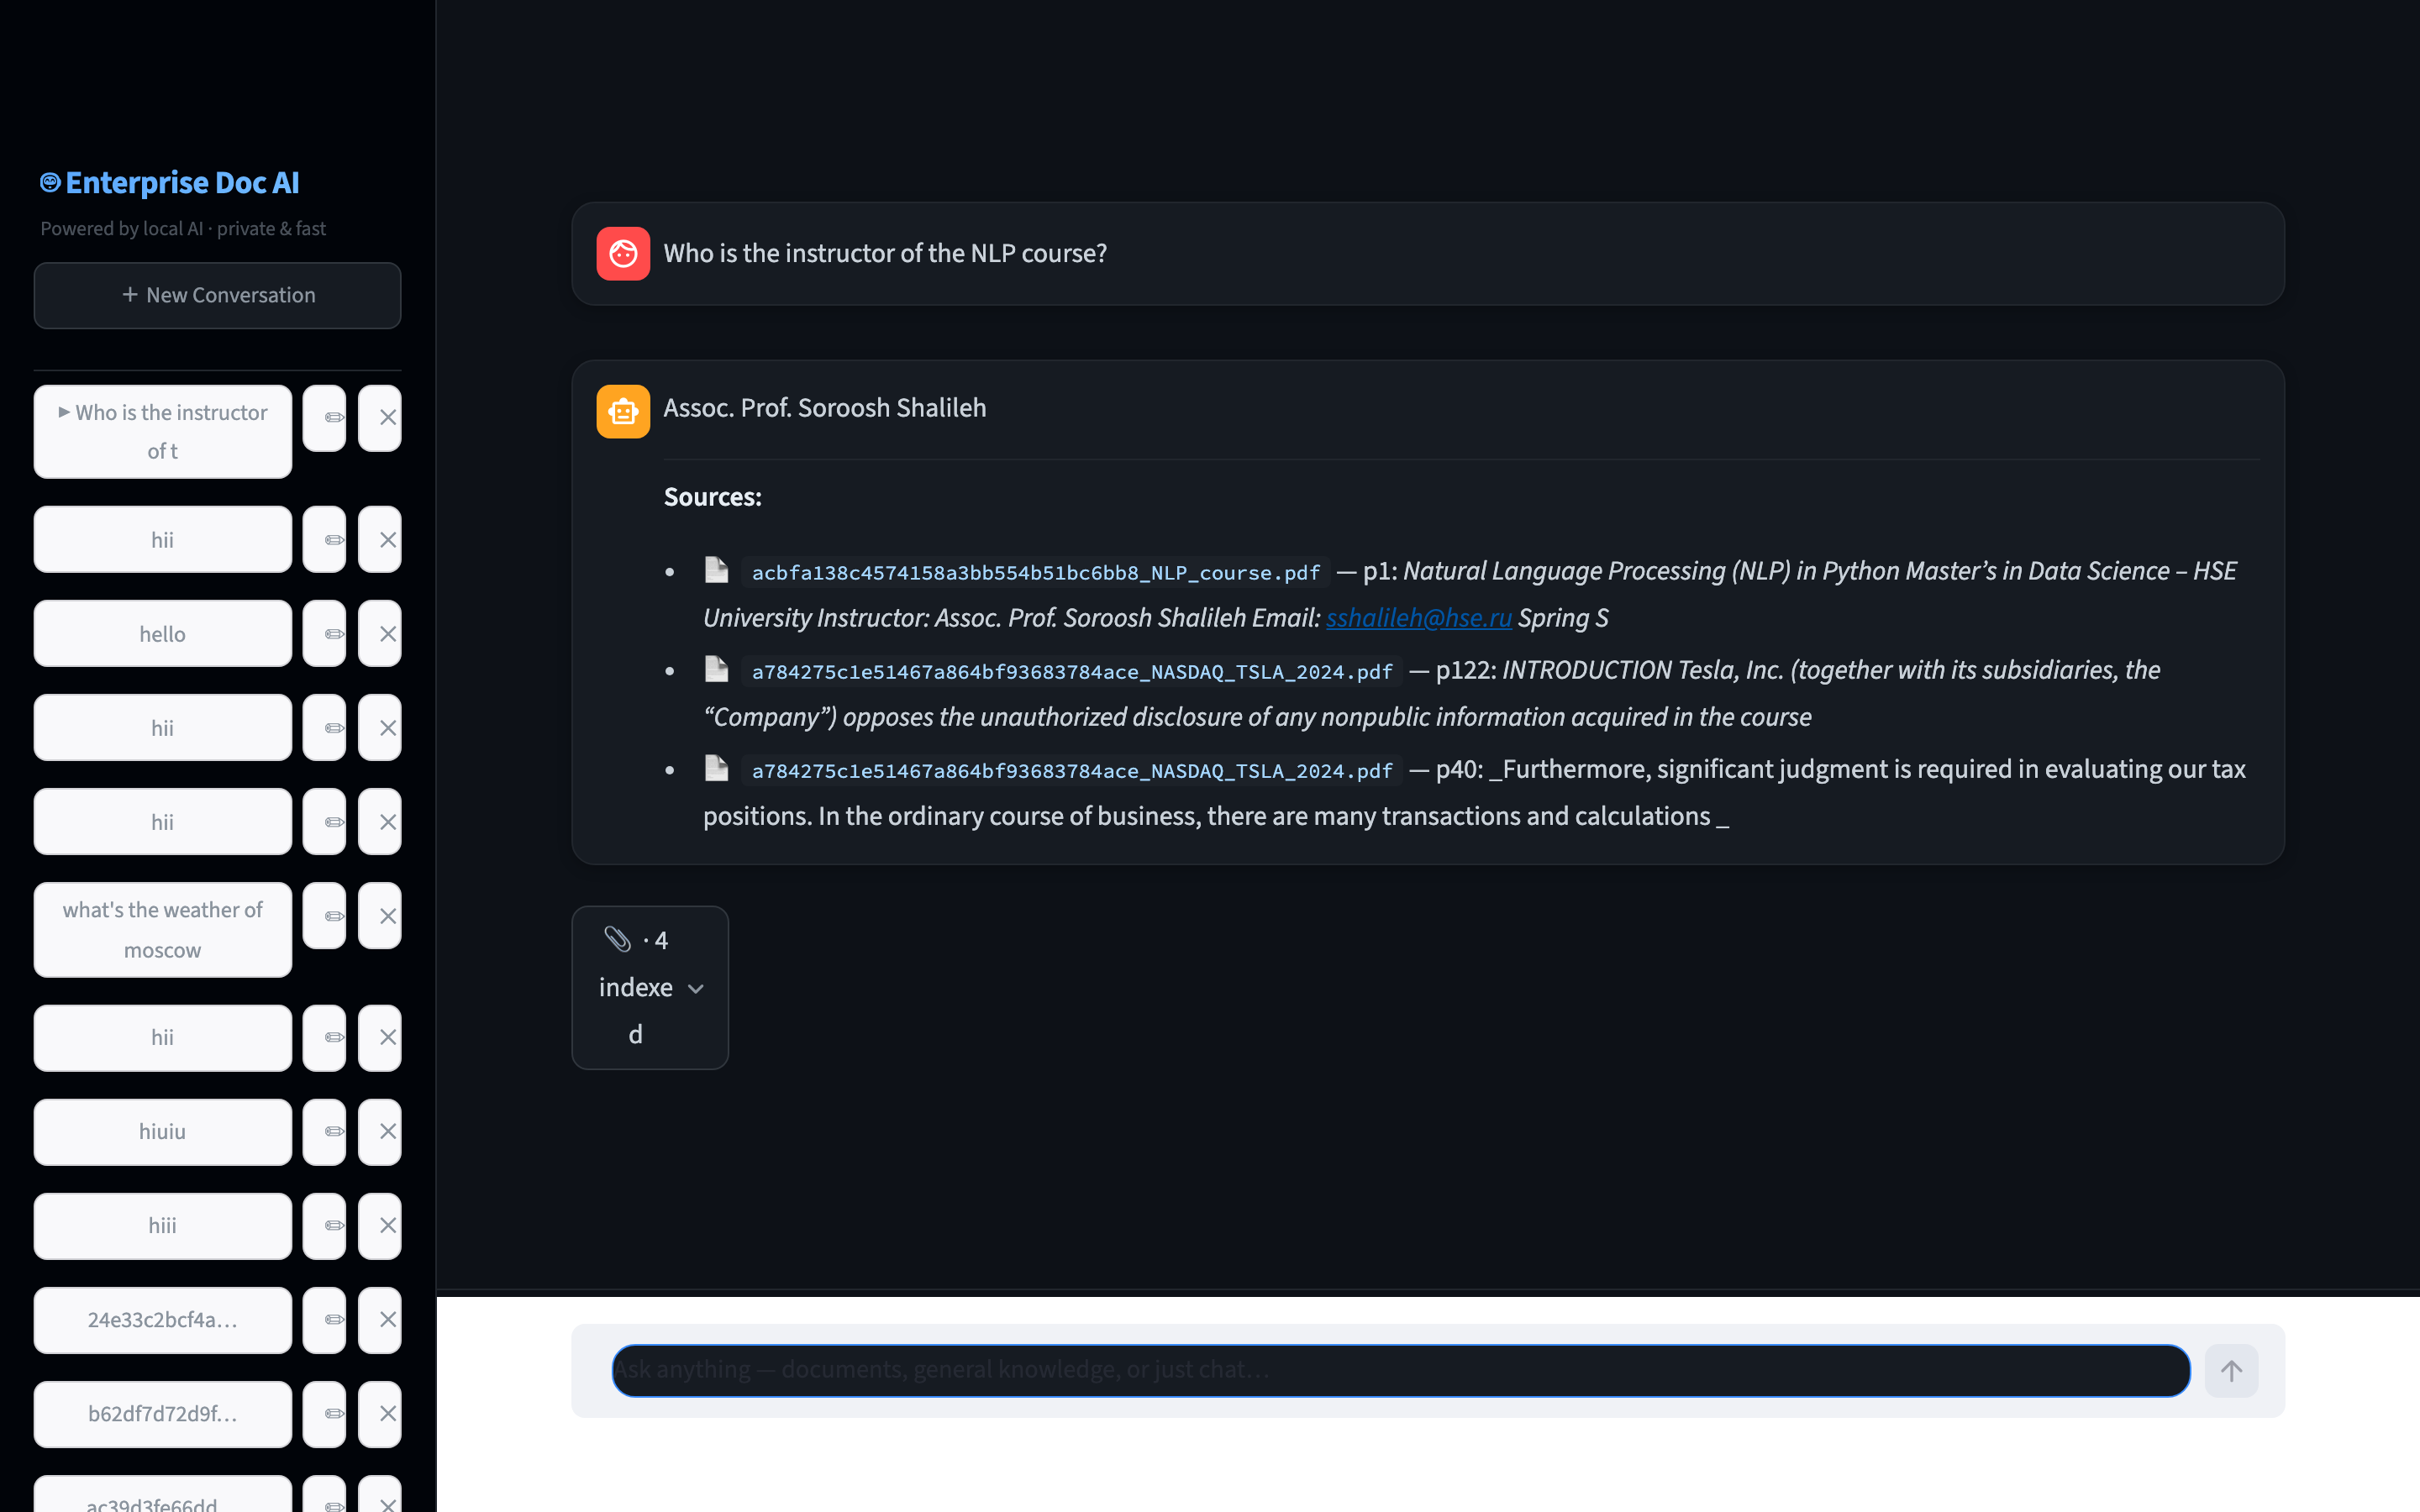
\includegraphics[width=\linewidth,height=5.7cm,keepaspectratio]{02_query_with_citations.png}\\[2pt]
{\scriptsize Grounded answer to a \textsc{factual} query, with three source citations
(file / page / snippet) rendered from chunk metadata.}
\end{column}
\end{columns}
\end{frame}

% --- Slide 9: Limitations & Future Work --------------------------------------
\begin{frame}{Limitations \& Future Work}
\textbf{Limitations}
\begin{itemize}\setlength{\itemsep}{1pt}
  \item \textbf{3\,B generator.} \texttt{llama3.2:3b} occasionally drops a correct retrieved
        fact in favour of a near-paraphrase; a 7\,--\,13\,B model would lift the answer-quality ceiling.
  \item \textbf{No cross-encoder rerank.} Hybrid lexical/dense fusion approximates it cheaply,
        but is weaker.
  \item \textbf{Rule-based router} can misclassify document queries that look superficially
        like ``ask the world'' questions.
\end{itemize}
\medskip

\textbf{Future work}
\begin{enumerate}\setlength{\itemsep}{1pt}
  \item \textbf{Cross-encoder rerank} (\texttt{bge-reranker-base} over top-20) --
        likely the single largest retrieval-quality lift.
  \item \textbf{Streaming responses} -- Ollama token-stream $\to$ FastAPI SSE $\to$ Streamlit.
  \item \textbf{Learned router} replacing the current rule-based router.
\end{enumerate}
\end{frame}

% --- Slide 10: Conclusion ----------------------------------------------------
\begin{frame}{Conclusion}
\begin{itemize}\setlength{\itemsep}{4pt}
  \item A fully \textbf{local-first} RAG system runs end-to-end on commodity laptop
        hardware, with no cloud or paid-API dependency.
  \item The engineering value lies in \emph{integration}: type-aware routing, LLM-bypass for
        the cheapest question types, table-aware chunking, and SQLite-as-source-of-truth.
  \item Result: a system a single user can run, understand, and \textbf{extend on their own
        hardware} -- the local-first counterpart to hosted RAG products.
\end{itemize}
\vfill
\centering
{\Large\textbf{Thank you. Questions?}}\\[6pt]
{\small\href{https://github.com/shahabazmi/intelligent-doc-qa}{github.com/shahabazmi/intelligent-doc-qa}}
\end{frame}

\end{document}
